\newpage
\subsection{Version control system}

\subsubsection{Git}
Git is a distributed revision control system. Initially designed and developed by Linus Torvalds 
it has now become one of the major and most popular revision control tools.
Git functions like a local version control for each user which can be linked to a common repository 
online to allow several participants to work together on one project. see figure ~\ref{fig:github}.

\begin{figure}[htb]
	\centering
	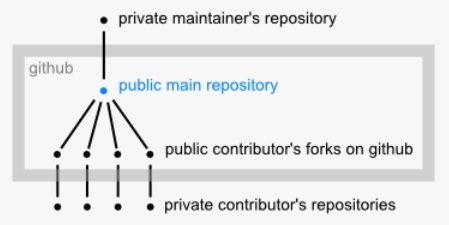
\includegraphics[width=0.6\textwidth]{organizational/github.jpg}
	\caption{Distributed setup of git repositories\cite{git:repositories}}
	\label{fig:github}
\end{figure}

\subsubsection{Reflection}
Because the project requires issue trackers and a rich commit history, the team has decided that using git is the right approach. The group has previous experience in using git, and we could get it up and running fairly quickly after project launch. The project is also Open Source, so having it as such on GitHub is not a problem.
